\documentclass[a4paper, 11pt]{article}

%Math
\usepackage{amsmath}
\usepackage{amsfonts}
\usepackage{amssymb}
\usepackage{amsthm}
\usepackage{ulem}
\usepackage{stmaryrd} %f\UTF{00FC}r Blitz!

%PageStyle
\usepackage[ngerman]{babel} % deutsche Silbentrennung
\usepackage[ansinew]{inputenc} % wegen deutschen Umlauten
\usepackage{fontenc}
\usepackage{fancyhdr, graphicx} %for header/footer
\usepackage{wasysym}
\usepackage{fullpage}
\usepackage{textcomp}

% Listings
\usepackage{color}
\usepackage{xcolor}
\usepackage{listings}
\usepackage{caption}

% Code listenings
\DeclareCaptionFont{white}{\color{white}}
\DeclareCaptionFormat{listing}{\colorbox{gray}{\parbox{\textwidth}{#1#2#3}}}
\captionsetup[lstlisting]{format=listing,labelfont=white,textfont=white}
 
\lstdefinestyle{JavaStyle}{
 language=Java,
 basicstyle=\footnotesize\ttfamily, % Standardschrift
 numbers=left,               % Ort der Zeilennummern
 numberstyle=\tiny,          % Stil der Zeilennummern
 stepnumber=5,              % Abstand zwischen den Zeilennummern
 numbersep=5pt,              % Abstand der Nummern zum Text
 tabsize=2,                  % Groesse von Tabs
 extendedchars=true,         %
 breaklines=true,            % Zeilen werden Umgebrochen
 frame=b,         
 %commentstyle=\itshape\color{LightLime}, Was isch das? O_o
 %keywordstyle=\bfseries\color{DarkPurple}, und das O_o
 basicstyle=\footnotesize\ttfamily,
 stringstyle=\color[RGB]{42,0,255}\ttfamily, % Farbe der String
 keywordstyle=\color[RGB]{127,0,85}\ttfamily, % Farbe der Keywords
 commentstyle=\color[RGB]{63,127,95}\ttfamily, % Farbe des Kommentars
 showspaces=false,           % Leerzeichen anzeigen ?
 showtabs=false,             % Tabs anzeigen ?
 xleftmargin=17pt,
 framexleftmargin=17pt,
 framexrightmargin=5pt,
 framexbottommargin=4pt,
 showstringspaces=false      % Leerzeichen in Strings anzeigen ?        
}

%Config
\renewcommand{\headrulewidth}{0pt}
\setlength{\headheight}{15.2pt}
\pagestyle{plain}

%Metadata
\title{Systemprogrammierung}
\author{Jan F�ssler}
\date{3. Semester (HS 2012)}
\fancyfoot[C]{If you use this documentation for a exam, you should offer a beer to the authors!}

% hier beginnt das Dokument
\begin{document}

% Titelbild
\maketitle
\thispagestyle{fancy}

\newpage

% Inhaltsverzeichnis
\pagenumbering{Roman}
\tableofcontents	  	


\newpage
\setcounter{page}{1}
\pagenumbering{arabic}

% Inhalt Start

\section{Unix/Linux}

\subsection{Aufbau}
\begin{center}
	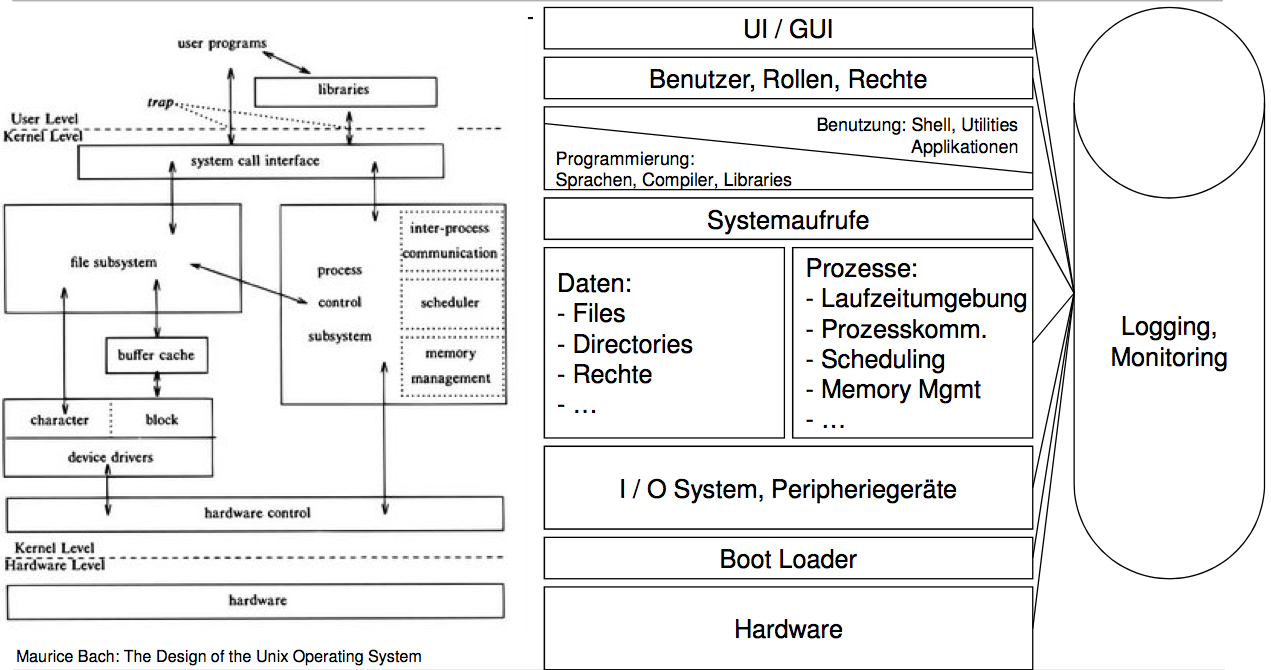
\includegraphics[scale=0.3]{aufbau-unix.png}
\end{center}

\subsection{Prozesse}
\subsubsection{Steuerungssystem}
\begin{itemize}
	\item Prozesse kreieren \& starten
	\item Prozesse schedulen, Warteschlangen, Ressourcenverbrauch
	\item Prozesse stoppen / unterbrechen / terminieren
	\item Prozess-Signalisierung und -kommunikation
	\item Faire Zuordnung von Hauptspeicher und anderen geteilten Ressourcen
	\item Ein-/Auslagerung von Prozessen bei vollem Speicher
	\item Prozesse und ihre Zust�nde anzeigen
\end{itemize}

\subsubsection{Aufbau}
\begin{center}
	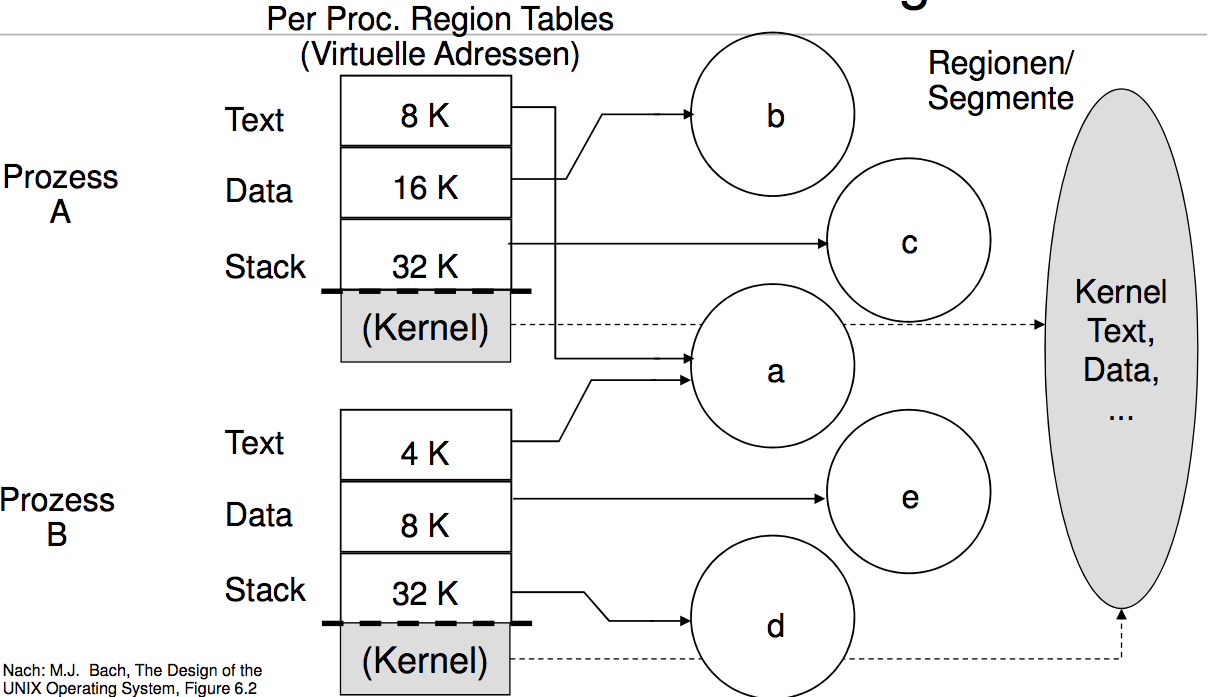
\includegraphics[scale=0.25]{prozess-aufbau.png}
\end{center}

\subsubsection{Kernel und User Mode}
\begin{itemize}
	\item Ein Prozess hat mindestens zwei Ausf�hrungsmodi:
		\begin{description}
			\item[User Mode] Es wird der normale Programmcode ausgef�hrt.
			\item[Kernl Mode] Es werden Systemaufrufe ausgef�hrt oder Ausnahmen behandelt.
		\end{description}
	\item Der �bergang erfolgt durch einen Systemaufruf durch das Programm, eine Ausnahmesituation oder durch asynchrone Events 
	\item Beide Modi haben separate Segmente und sind voneinander abgeschirmt.
\end{itemize}

\subsubsection{Zust�nde}
\begin{center}
	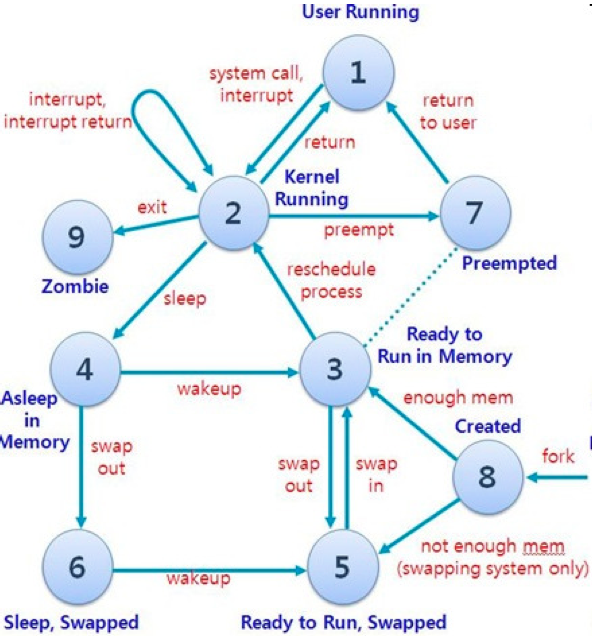
\includegraphics[scale=0.5]{process-states.png}
\end{center}

\subsection{Memory}
\subsubsection{Virtual Memory}
\begin{itemize}
	\item Erweiterung des Hauptspeichers pro System (mehr Prozesse im System als Speicher verf�gbar), oder pro Prozess (einzelner Prozess gr�sser als verfu?gbarer Hauptspeicher).
	\item Systematische Abstraktion fu?r systemspezifische Overlay- Techniken.
	\item Organisation des Hauptspeichers in gleich grosse, einheitlich adressierbare Einheiten.
\end{itemize}

\subsubsection{Swapping}
\begin{center}
	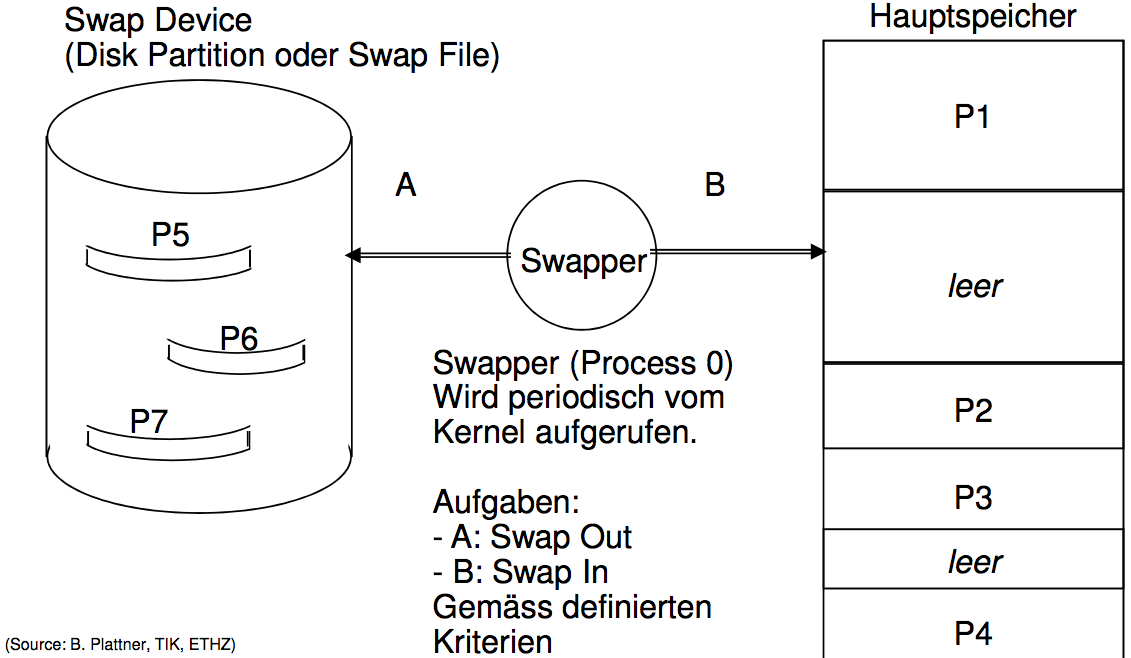
\includegraphics[scale=0.3]{swapping.png}
\end{center}

\subsubsection{Paged Memory}
Design und Layout der Datenstrukturen fu?r die seiten-orientierte Speicherverwaltung variieren zwischen Unix- und Linux-Varianten und sind zudem von den Hardware- Eigenschaften abh�ngig. Linux verwendet zum Beuispiel eine 3-stufige Seitentabelle:
\begin{itemize}
	\item Page Directory pro Prozess und f�r den BS-Kern
	\item Page Mid-level Directory (f�r 64 bit CPU-Architekturen) Paged Memory II
	\item Page Table, enth�lt Seitenbeschreibungen und Verweise auf den physische Speicheror
\end{itemize}

\subsubsection{Fehlerzust�nde}
\begin{center}
	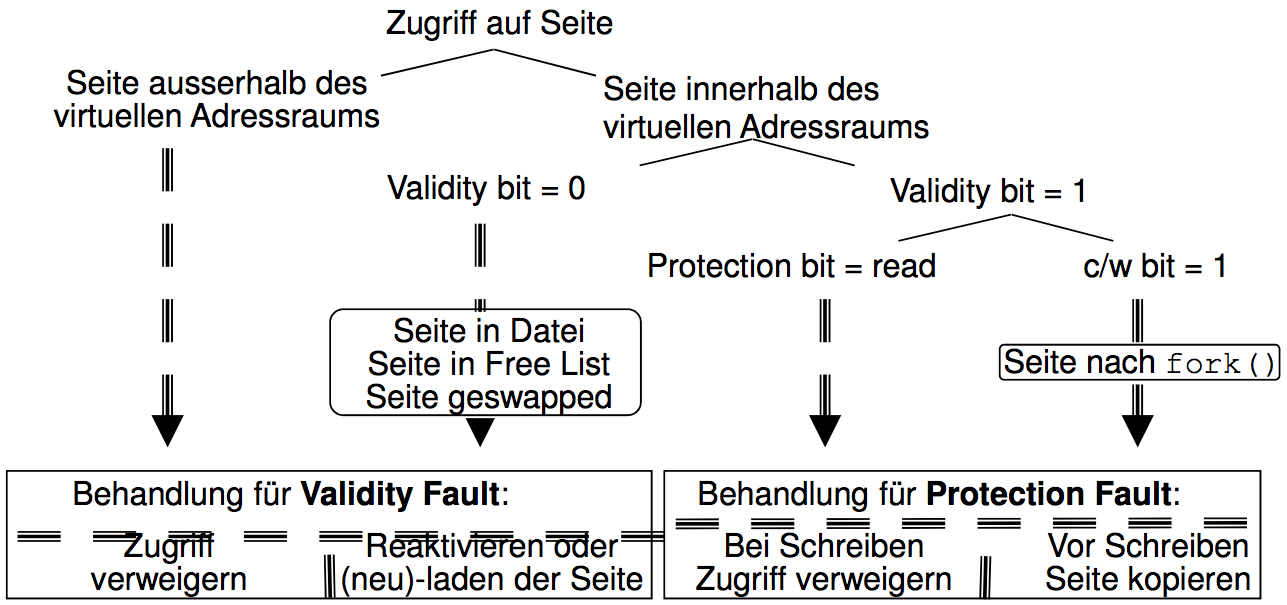
\includegraphics[scale=0.3]{memory-error-state.png}
\end{center}

\newpage
\section{System Call Schnittstelle}
\begin{center}
	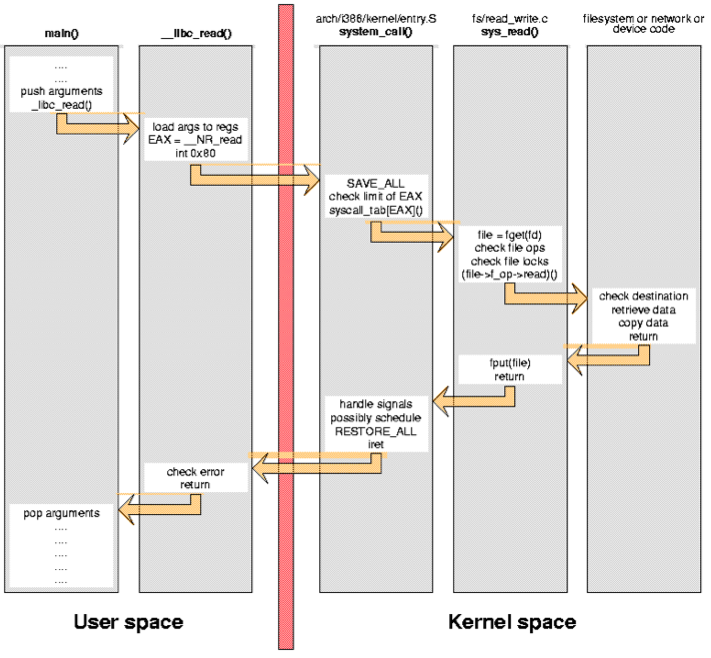
\includegraphics[scale=0.5]{system-calls.png}
\end{center}
\subsection{Prozess-System}
\begin{description}
	\item[fork()] Erzeugung
	\item[exit()] Beendigung
	\item[exec()] �berlagerung des Prozesses
	\item[wait()] Warten auf Prozesstermination (Kindprozesse)
	\item[sleep()] Freiwilliges schlafen des Prozesses.
	\item[kill()] Senden eines Signals (32 verschiedene)
	\item[signal()] Signalbehandlung
\end{description}

\subsection{Datei-System}
\begin{description}
	\item[creat()] Anlegen einer Datei
	\item[mknod()] Anlegen eines Ordners
	\item[open()] �ffnen einer Datei
	\item[close()] Schliessen einer Datei
	\item[unlink()] L�schen einer Datei
	\item[read()] Lesen aus einer Datei
	\item[write()] Schreiben in eine Datei
	\item[lseek()] Vorw�rts-/R�ckwertsbewegung
	\item[ioctl()] Kontrollieren der Eigenschaften
	\item[dup()] Duplizieren eines Dateideskriptors
	\item[chown, chmod, umask] Zugriffsrechte
	\item[chdir()] Navigation im Dateisystem
\end{description}

\subsection{Directory Handling}
\begin{description}
	\item[opendir()] �ffnen eines Verzeichnises
	\item[readdir()] Lesen eines Verzeichnises
	\item[writedir()] Schreiben eines Verzeichnises
	\item[closedir()]  Schliessen eines Verzeichnises
\end{description}
		
\subsection{Speicherverwaltung}
\begin{description}
	\item[malloc()] Speicher allozieren
	\item[free()	] Speicher freigeben
\end{description}

\subsection{Weitere}
\begin{description}
	\item[pipe()] Basis-Interprozesskommunikation
	\item[socket()] Interprozesskommunikation lokal oder u?ber Netzwerke
\end{description}
% Inhalt Ende
\end{document}